\section{Numerical Experiments}
\label{sec:experiments}

This section has two purposes. Section~\ref{sec:bound-validation} evaluates the rule-level upper bound on the platooning-induced optimality gap. Section~\ref{sec:pp-validation} evaluates the proposed platooning method against no platooning and conventional critical-headway platooning. The two studies use the same traffic generator and parameter grid, but they answer different questions and use different solver-time protocols.

\subsection{Validation of the Rule-Level Upper Bound}
\label{sec:bound-validation}

\subsubsection{Experiment Setting}
\label{sec:bound-setting}

We consider a general conflict area with four single-lane approaches. The total number of vehicles is varied over
\begin{equation}
N\in\{20,40,60,80\}.
\end{equation}
Vehicles are distributed as evenly as possible across the four approaches. Vehicle arrivals on each approach are generated independently according to a Poisson process with arrival rate
\begin{equation}
\lambda\in\{0.4,0.7,1.0\}\ \text{veh/s}.
\end{equation}
The minimum following and switching headways are fixed at \(\hF=1\)~s and \(\hS=3\)~s, respectively. The platooning threshold and maximum platoon size are varied over
\begin{equation}
\delta\in\{2,4,6,8\}\ \text{s},
\qquad
P_{\max}\in\{2,4,6,8\}.
\end{equation}
For each combination of \(N\), \(\lambda\), \(\delta\), and \(P_{\max}\), we generate 20 independent traffic instances.

For each instance, the no-platooning model is solved to obtain the reference delay \(D_{\mathrm{NP}}\). The proposed platooning rule is then applied and the resulting platoon-level model is solved to obtain \(D_{\mathrm{PP}}\). The realized platooning-induced optimality gap is
\begin{equation}
G(\Pi)=D_{\mathrm{PP}}-D_{\mathrm{NP}}.
\end{equation}
A bound check is performed only when both the NP and PP models are proven optimal. The empirical validation therefore checks
\begin{equation}
G(\Pi)\le \widehat G(\delta,P_{\max})
\end{equation}
only on the subset of cases with an exact NP reference. NP models that do not prove optimality within the initial 30-second run are rerun in a recovery stage with a 600-second limit. All models use 12 Gurobi threads. The recovery results are used only to increase the number of exact gap checks; the 30-second results remain the basis for the fixed-budget computation comparison in Section~\ref{sec:pp-validation}.

\begin{table}[t]
  \centering
  \caption{Experiment settings for validating the rule-level upper bound.}
  \label{tab:bound-setting}
  \begin{tabular}{ll}
    \toprule
    Parameter & Value \\
    \midrule
    Number of approaches \(L\) & 4 \\
    Total number of vehicles \(N\) & \(20,40,60,80\) \\
    Arrival rate \(\lambda\) & \(0.4,0.7,1.0\) veh/s \\
    Minimum following headway \(\hF\) & 1 s \\
    Minimum switching headway \(\hS\) & 3 s \\
    Platooning threshold \(\delta\) & \(2,4,6,8\) s \\
    Maximum platoon size \(P_{\max}\) & \(2,4,6,8\) \\
    Replications & 20 \\
    Gurobi threads & 12 \\
    Initial time limit & 30 s per model \\
    NP recovery limit & 600 s per unresolved NP model \\
    \bottomrule
  \end{tabular}
\end{table}

\subsubsection{Results}
\label{sec:bound-results}

This subsection will report the number and coverage of valid bound checks, the number of observed violations, the realized gap, the rule-level upper bound, and the bound slack. The bound is interpreted as a worst-case guarantee rather than a point prediction of the realized gap.

\begin{figure}[t]
  \centering
  \IfFileExists{figures/bound_validation_actual_vs_upper.pdf}{
    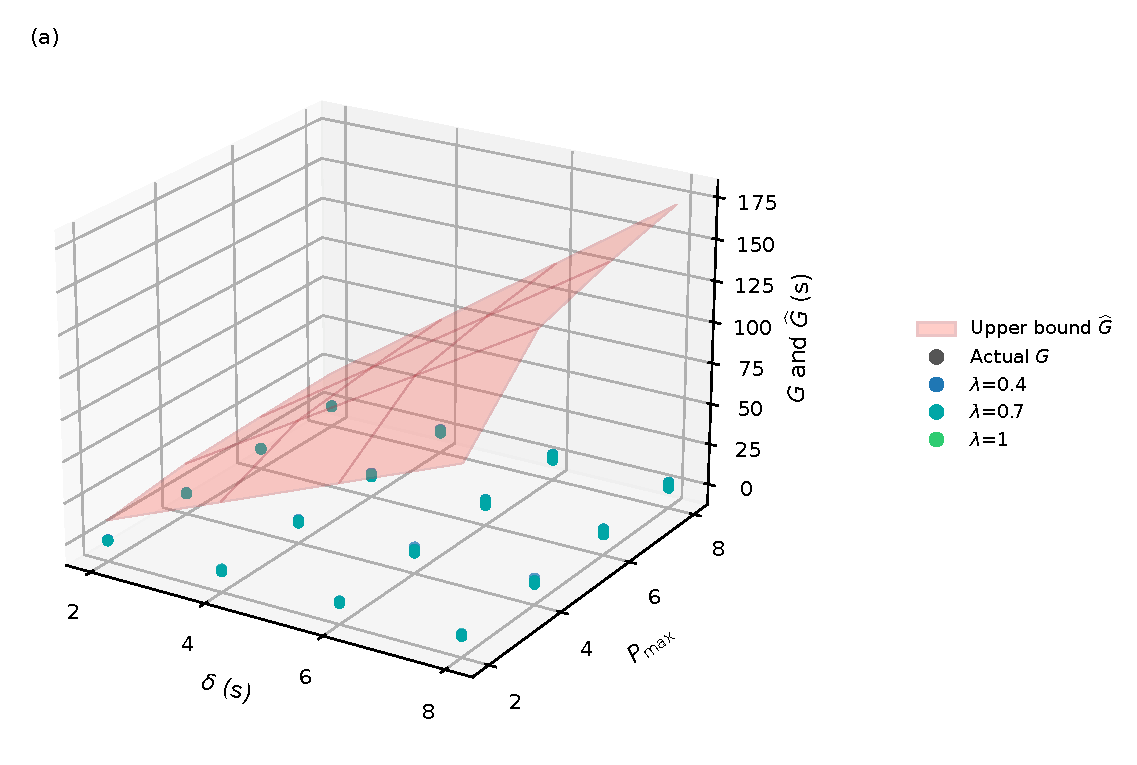
\includegraphics[width=0.78\textwidth]{figures/bound_validation_actual_vs_upper.pdf}
  }{
    \fbox{\parbox[c][0.25\textheight][c]{0.72\textwidth}{\centering Placeholder for the final bound-validation figure.\\Actual \(G\) and rule-level upper bound \(\widehat G\).}}
  }
  \caption{Actual platooning-induced optimality gap \(G\) and the rule-level upper bound \(\widehat G(\delta,P_{\max})\) under different platooning thresholds and maximum platoon sizes. Colors represent \(\delta\), and marker shapes represent \(P_{\max}\). Only cases with proven-optimal NP and PP solutions are included.}
  \label{fig:bound-validation}
\end{figure}

\begin{figure}[t]
  \centering
  \IfFileExists{figures/experimental_tradeoff_solve_time_gap.pdf}{
    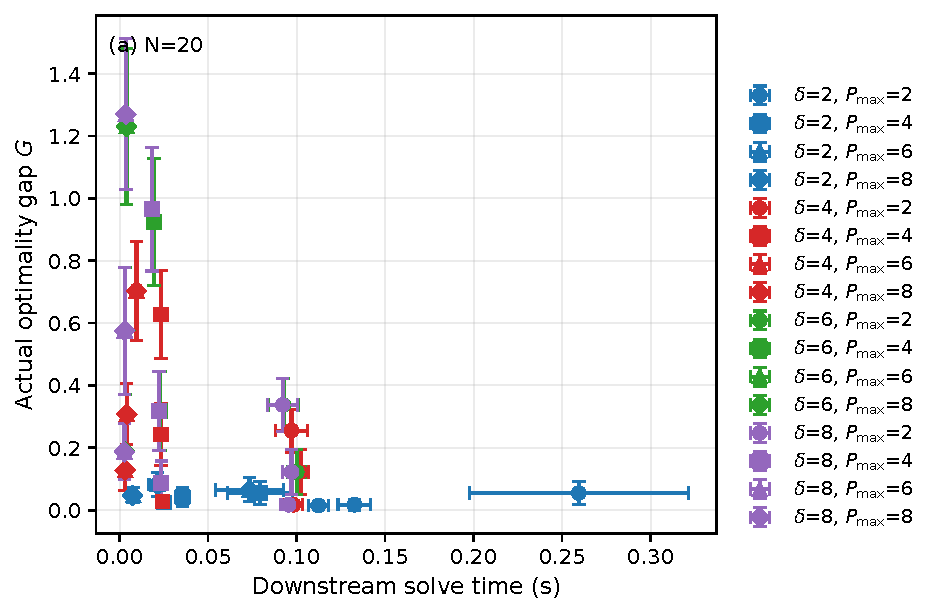
\includegraphics[width=0.78\textwidth]{figures/experimental_tradeoff_solve_time_gap.pdf}
  }{
    \fbox{\parbox[c][0.25\textheight][c]{0.72\textwidth}{\centering Placeholder for the final experimental trade-off figure.\\Solve time versus actual gap \(G\).}}
  }
  \caption{Trade-off between downstream solve time and the actual platooning-induced optimality gap \(G\). Colors represent \(\delta\), and marker shapes represent \(P_{\max}\).}
  \label{fig:experimental-tradeoff}
\end{figure}

\subsection{Validation of the Proposed Platooning Method}
\label{sec:pp-validation}

\subsubsection{Experiment Setting}
\label{sec:pp-setting}

The second study compares three methods on the same instances: NP treats every vehicle as an independent scheduling unit; CHP applies a conventional critical-headway rule using \(\delta\) without a platoon-size cap; and PP applies the proposed rule using both \(\delta\) and \(P_{\max}\). The traffic settings are identical to Table~\ref{tab:bound-setting}, with \(N\in\{20,40,60,80\}\), \(L=4\), \(\lambda\in\{0.4,0.7,1.0\}\), \(\hF=1\)~s, \(\hS=3\)~s, \(\delta\in\{2,4,6,8\}\), and \(P_{\max}\in\{2,4,6,8\}\). Each configuration uses 20 independent replications.

All three methods use the same 30-second downstream time limit and 12 Gurobi threads. NP is solved once per instance, CHP once for each \(\delta\), and PP once for each \((\delta,P_{\max})\). The comparison reports average vehicle delay, incumbent objective, optimality rate, terminal MIP gap, number of scheduling units, dimension-reduction ratio, solve time, end-to-end time, and branch-and-bound node count. The delay ordering
\begin{equation}
D_{\mathrm{NP}}\le D_{\mathrm{PP}}\le D_{\mathrm{CHP}}
\end{equation}
is checked only when all three corresponding models are proven optimal. For larger time-limited NP cases, objective, status, MIP gap, runtime, and node count are reported without claiming knowledge of the true optimality gap.

\begin{table}[t]
  \centering
  \caption{Experiment settings for comparing NP, CHP, and PP.}
  \label{tab:pp-setting}
  \begin{tabular}{ll}
    \toprule
    Parameter & Value \\
    \midrule
    Methods & NP, CHP, PP \\
    Number of approaches \(L\) & 4 \\
    Total number of vehicles \(N\) & \(20,40,60,80\) \\
    Arrival rate \(\lambda\) & \(0.4,0.7,1.0\) veh/s \\
    Minimum following headway \(\hF\) & 1 s \\
    Minimum switching headway \(\hS\) & 3 s \\
    Platooning threshold \(\delta\) & \(2,4,6,8\) s \\
    Maximum platoon size \(P_{\max}\) & \(2,4,6,8\) \\
    Replications & 20 \\
    Time limit & 30 s per downstream model \\
    Gurobi threads & 12 \\
    \bottomrule
  \end{tabular}
\end{table}

\subsubsection{Results}
\label{sec:pp-results}

This subsection will first compare the delay performance of NP, CHP, and PP. It will then explain the computational mechanism through changes in the number of platoons, downstream model dimension, solve time, and fixed-time solver behavior.

\begin{figure}[t]
  \centering
  \IfFileExists{figures/pp_delay_vs_threshold_density.pdf}{
    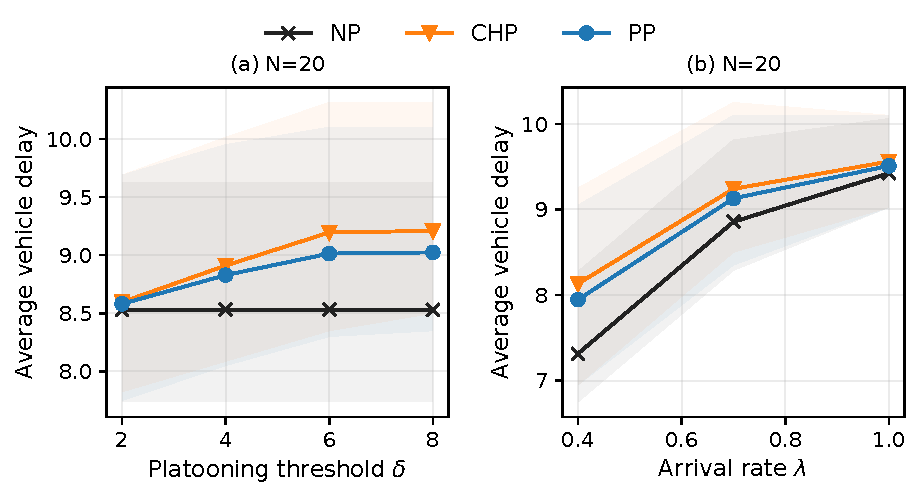
\includegraphics[width=0.88\textwidth]{figures/pp_delay_vs_threshold_density.pdf}
  }{
    \fbox{\parbox[c][0.27\textheight][c]{0.80\textwidth}{\centering Placeholder for the PP delay comparison.\\Panel (a): delay versus \(\delta\). Panel (b): delay versus \(\lambda\).}}
  }
  \caption{Average vehicle delay of NP, CHP, and PP as the platooning threshold or vehicle arrival rate increases. Panel (a) varies \(\delta\), and Panel (b) varies \(\lambda\).}
  \label{fig:pp-delay}
\end{figure}

\begin{figure}[t]
  \centering
  \IfFileExists{figures/pp_time_and_platoon_count.pdf}{
    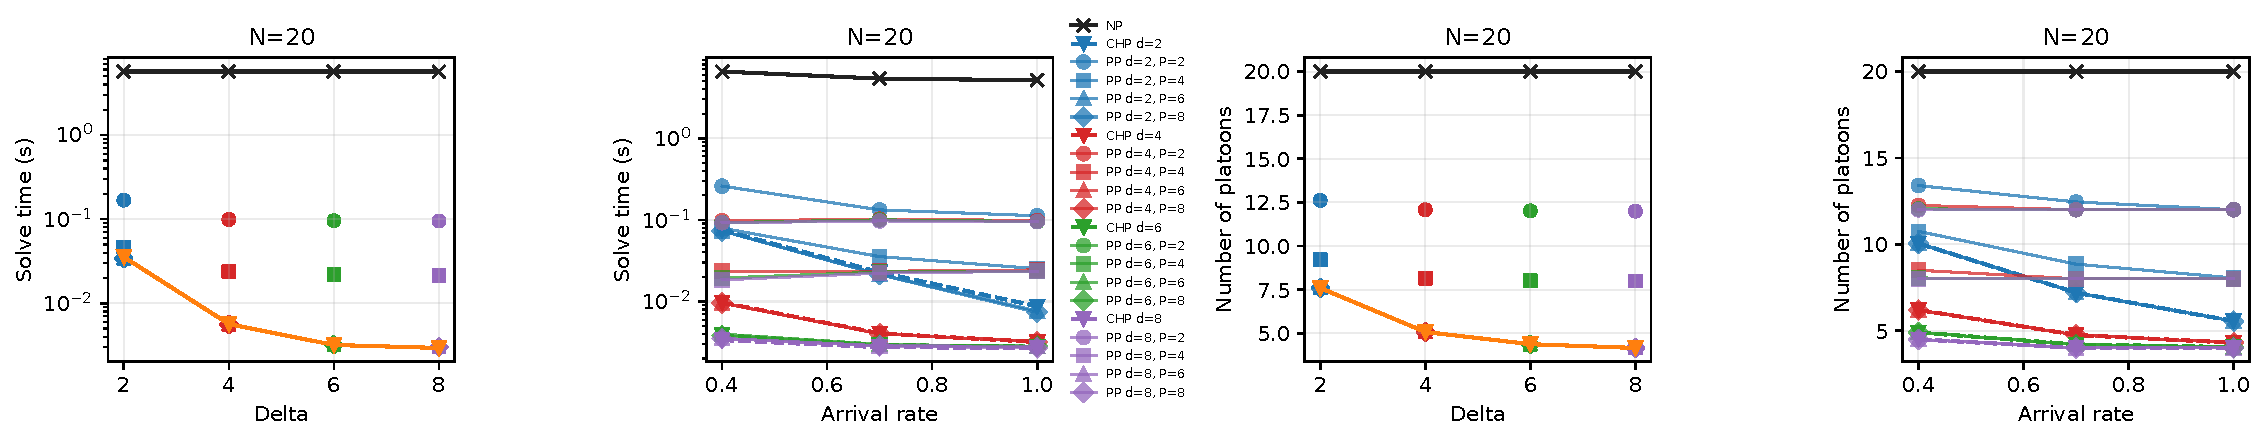
\includegraphics[width=0.92\textwidth]{figures/pp_time_and_platoon_count.pdf}
  }{
    \fbox{\parbox[c][0.34\textheight][c]{0.84\textwidth}{\centering Placeholder for the PP computation-mechanism figure.\\Solve time and number of platoons versus \(\delta\) and \(\lambda\).}}
  }
  \caption{Solution time and number of scheduling units for NP, CHP, and PP. The panels show how both quantities change with the platooning threshold and vehicle arrival rate.}
  \label{fig:pp-time-platoons}
\end{figure}

\begin{figure}[t]
  \centering
  \IfFileExists{figures/gurobi_solution_quality_over_time.pdf}{
    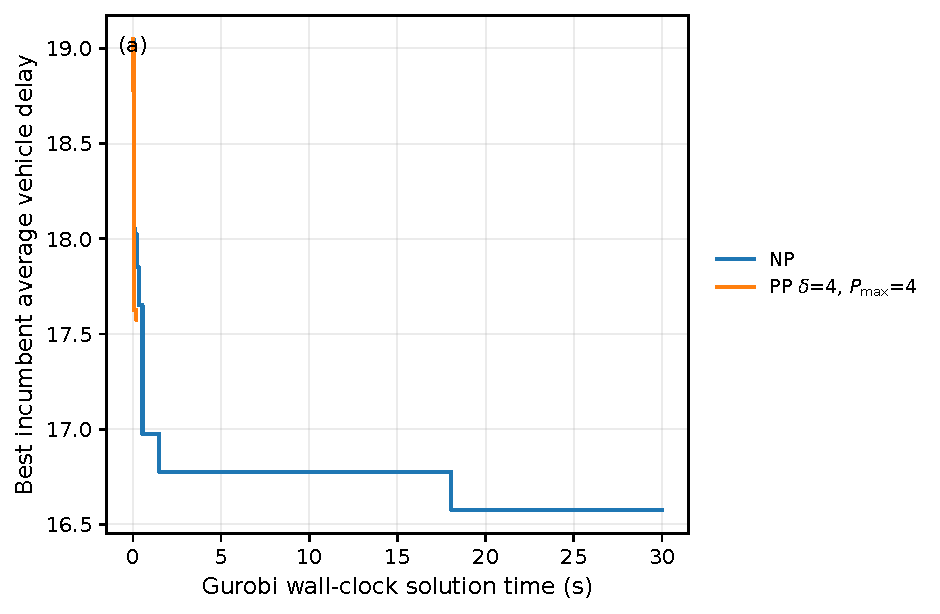
\includegraphics[width=0.82\textwidth]{figures/gurobi_solution_quality_over_time.pdf}
  }{
    \fbox{\parbox[c][0.27\textheight][c]{0.76\textwidth}{\centering Placeholder for the Gurobi incumbent trajectory figure.\\Best-found solution quality versus wall-clock time.}}
  }
  \caption{Quality of Gurobi solutions as a function of wall-clock time for NP, CHP, and representative PP parameter settings. The figure illustrates the practical value of dimension reduction under a limited computation budget.}
  \label{fig:gurobi-quality-time}
\end{figure}
